\section{Preliminary Results} \label{sec:preliminaries}

\subsection{The Production Network}


\begin{figure}[t]
    \centering
    \subfigure[Product Graph \label{subfig:product_graph}]{
    \begin{tikzpicture}[transform shape,scale=0.65]
        \Vertex[x=-1, y=-1]{u1}
        \Vertex[x=-1, y=0]{u2}
        \Vertex[x=-1, y=1]{u3}
        \Text[x=-1, y=-2, fontsize=\scriptsize]{Raw Materials ($d = D$)}

        \Vertex[x=1, y=-0.5]{v1}
        \Vertex[x=1, y=0.5]{v2}
        

        \Edge[Direct, color=black](u1)(v1)
        \Edge[Direct, color=black](u3)(v1)
        
        \Edge[Direct, color=black](u2)(v2)
        \Edge[Direct, color=black](u1)(v2)
        
        \Text[x=2, y=0]{$\dots$}
        
        \Vertex[x=5, y=-1]{w1}
        \Vertex[x=5, y=0]{w2}
        \Vertex[x=5, y=1]{w3}
        \Text[x=5, y=-2, fontsize=\scriptsize]{Specialized Products ($d = 1$)}
        
        \Vertex[x=3, y=0.5]{z1}
        \Vertex[x=3, y=-0.5]{z2}
        
        \Edge[Direct, color=black](z1)(w1)
        \Edge[Direct, color=black](z1)(w2)
        \Edge[Direct, color=black](z1)(w3)
        
        \Edge[Direct, color=black](z2)(w1)
        \Edge[Direct, color=black](z2)(w2)
        \Edge[Direct, color=black](z2)(w3)
        
        
    \end{tikzpicture}}
    \subfigure[Supplier Set \label{subfig:suppliers}]{
    \begin{tikzpicture}[multilayer=3d,transform shape,scale=0.55]
    \Vertex[x=0, y=0, layer=1, label=$i$]{i}
    
    
    \Vertex[x=0, y=-1, color=teal, opacity=0.7, layer=2]{S1}
    \Vertex[x=0, y=0, color=teal, opacity=0.7, layer=2]{S2}
    \Vertex[x=0, y=1, color=teal, opacity=0.7, layer=2]{S3}
    
    \Edge[Direct, style=dashed, label=$x$](S1)(i)
    \Edge[Direct, style=dashed, label=$x$](S2)(i)
    \Edge[Direct, style=dashed, label=$x$](S3)(i)
    \Text[x=-2, y=3.5]{$\cS(i)$}
    
    \Plane[x=-0.5,y=-2,width=1,height=4, layer=2, color=teal]
    
    \end{tikzpicture}}
    \caption{Supply-chain Instance.}

    \label{fig:supply_chain}
\end{figure}


We start by describing the production network.  We consider the production of a set of products $\cK$ with cardinality $|\cK| = K$ where each product $i \in \cK$ can be produced by a number of suppliers and also requires certain inputs in order to be produced. Specifically, each product $i \in \cK$ has a set of requirements (inputs), denoted by $\cN(i)$ that it needs in order to be made. The products and the set of requirements for each product define the \emph{production network} $\cG = \cG(\cV(\cG) = \cK, \cE(\cG))$. 

The production network $\cG$ contains \emph{raw materials} (or sources), which are materials that do not require any inputs, i.e., have $|\cN(i)| = 0$ and are the ``initial products'' that are used in the production of others. We denote the set of raw materials as $\cR \subseteq \cK$. Each product $i \in \cK$ can be sourced from a set of suppliers $\cS(i)$. We assume that a supplier of a product can source from \emph{any} supplier of a product that the supplier depends on (one may argue here that it is impossible that every supplier of a product $i$ can source from every supplier of, say, product $j$, due to geographical constraints. The issue can be mitigated by expanding vertex $j$ to multiple sub-nodes).

% \begin{definition*}[Supplier Graph]
%     The supplier graph $\cH$ is defined to be a graph with vertex set $\cV(\cH) = \bigcup_{i \in \cK} \cS(i)$ and edge set $\cE(\cH) = \bigcup_{i \in \cK} \bigcup_{j \in \cN(i)} \cB(\cS(i), \cS(j))$, where $\cB(\cS(i), \cS(j))$ is the complete bipartite graph between $\cS(i)$ and $\cS(j)$.  
% \end{definition*}

For simplicity, throughout the rest of the paper, we will assume that $|\cS(i)| = n$ for all $i \in \cK$.

\noindent \textbf{Structural Assumptions on $\cG$.} For our main results, we make the structural assumption that the production network $\cG$ is a Directed Acyclic Graph (DAG), i.e., a natural order exists among the products being produced, i.e., the production of more complex products depends on sourcing inputs from simpler products. Such an assumption has appeared in prior work, e.g., \citet{elliott2022supply,blaettchen2021traceability,bimpikis2019supply}. Later in the paper (\cref{sec:general_supply_chains}), we show how we can relax this assumption and allow for cycles $\cG$.

% \noindent \textbf{Example.} Assume a simple network that produces $\cK = \{  \text{engines}, \text{bolts}, \text{screws} \}$. We have, e.g. $\cN(\text{engines}) = \{ \text{bolts}, \text{screws} \}$ and $\cS(\text{engines}) = \{ \text{BMW}, \text{General Motors} \}$, and suppliers for the screws and bolts.

\noindent \textbf{Additional Notation.} We use $[K]$ to denote the set $\{ 1, \dots, K \}$. 
For vectors (resp. matrices), we use $\| x \|_p$ for the $p$-norm of $x$ (resp. for the induced $p$-norm); for the Euclidean norm (i.e., $p = 2$), we omit the subscript. $\zero$ (resp. $\one$) denotes all zeros (resp. all ones) column vector, and $\one_S$ represents the indicator column vector of the set $S$. 
We use $x \wedge y$ (resp. $x \vee y$) as shorthand for the coordinate-wise minimum (resp. maximum) of vectors $x$ and $y$.
Finally order relations $\ge, \le, >, <$ denote coordinate-wise ordering.  $\mathsf{vec}(A)$ corresponds to the vectorization of matrix $A$. We use $\cG^R$ to denote the reverse graph of $\cG$, i.e., the graph which has the same vertex set as $\cG$ and reversed edges. In our context, $\cG$ corresponds to the graph of supply relations, and $\cG^R$ corresponds to the graph of source relations. The notation $\{ y_n \}_{n \in \Nbb}$ the notation $x_n \asymp y_n$ means that $\lim_{n \to \infty} \frac {x_n} {y_n} = 1$. 


% \mpcomment{talk about modelling assumptions on the production network and how they can model a wide range of phenomena such as geographically separate groups of suppliers}

\subsection{Node Percolation} \label{sec:node_percolation}

The supply chain graph $\cG$ undergoes a node percolation process at which each supplier fails independently at random with probability $x \in (0, 1)$. Each product can be produced if, and only if, \emph{(i)} all of its requirements $j \in \cN(i)$ can be produced, and, \emph{(ii)} at least one of the suppliers $s \in \cS(i)$ is operational. Upon the completion of the percolation process, a random number $F$ of products fails, and the remaining $S = K - F$ products survive. The number of surviving products can be expressed as  $S = \sum_{i \in \cK} Z_i$ where $\{ Z_i \}_{i \in \cK}$ are the indicator variables that equal to one if, and only if, product $i$ is produced and are zero otherwise. The sequence of variables $\{ Z_i \}_{i \in \cK}$ obeys the following random system of equations for every $i \in \cK$:
\begin{align} \label{eq:dynamics} 
    Z_i & = \prod_{j \in \cN(i)} Z_j \left ( 1 - \prod_{s \in \cS(i)} Y_{is} \right ), 
    % Y_{is} & \sim \mathrm{Be} (x) & \quad \forall s \in \cS(i) \nonumber \\
    % Y_{is} & \perp Y_{i's'} & \quad \forall i \neq i', s \neq s'. \nonumber
\end{align} where $Y_{is} \overset  {\mathsf{i.i.d.}} {\sim} \mathrm{Be}(x)$ for all $i \in \cK, s \in \cS(i)$.  Our paper aims to study the random behavior of $F$ (resp. $S$). A planner is interested in finding the maximum probability value $x$ such that the number of failures is at most $\varepsilon K$ (e.g., sublinear) with high probability. We show that some very simple production networks can experience power-law cascades to motivate such a resilience metric. 

\subsection{Motivation for a Resilience Metric: Cascading failures and the emergence of power laws in random DAG structures} \label{sec:motivation}

% \begin{figure}[t]
%     \centering
    

%     \caption{Illustration of $\mathsf{rdag}(K = 3, p)$ with failures drawn in pink.}
%     \shrink
%     \label{fig:random_dag_2}
% \end{figure}

We start by motivating the need for the definition of a resilience measure for supply chain graphs. More specifically, similarly to large social networks \citep{leskovec2007patterns,wegrzycki2017cascade} and power networks \citep{dobson2004branching,dobson2005loading,nesti2020emergence}, we show that a randomly generated supply chain with random DAG structure exhibits cascades that obey a power law, namely the average cascade size is dominated by a few very large scale cascades rather than the many smaller ones. 

In a supply chain, we can assume that there is a ``natural order'' among the products being produced; namely, the production of more complex products is contingent on supplying simpler products. In a supply chain, raw materials and component parts are typically transformed into intermediate products and then into finished products through a series of production processes. The production of more complex products often depends on the availability of simpler products, as the simpler products are used as inputs in the production of the more complex products. For example, in the production of a car, the production of the car's engine may depend on the availability of simpler components such as computer chips. In its simplest form, this kind of behavior can be captured by a random DAG model, where a DAG is created by independently sampling edges via coin tosses. %Similarly, the production of the car's body may depend on the availability of the car's engine, as well as other intermediate products such as doors and windows.  

To observe this, we start with the random DAG model $\mathsf{rdag}(K, p)$ described in the work of \citet{wegrzycki2017cascade}. More specifically, we consider a supply chain with $K$ products $i_1, \dots, i_K$ connected as follows: for every $k \in [K]$ and for every $1 \le l \le K - 1$ we add a directed edge $(i_l, i_k)$ independently with probability $p \in (0, 1)$. \cref{fig:random_dag_2} shows the creation of a $\mathsf{rdag}(K, p)$ with probability $p$ and $K = 3$ vertices.

% \mar{It would be good to motivate the random DAG model for production networks, e.g., there is a natural order among products where production of more complex products is contingent on supplies of  simpler products}. 

The percolation process happens as described in \cref{sec:node_percolation}. The following theorem determines the distribution of the failure cascade size $F$ and shows that it grows at least as a power law with exponent one. Our proof follows similar arguments as those made by \citet{wegrzycki2017cascade}. 

\begin{theorem} \label{theorem:power_laws}
    Let $G \sim \mathsf{rdag}(K, p)$ be the production network of $K$ products that is realized according to a random DAG model, and consider the node percolation model with failure probability $x$ on the supplier graph associated with the production network $G$. Then $\Pr[F = f] \asymp \frac {x^n} {K(1 - (1 - x^n)(1 - p)^f)} \ge \frac {C(K, p, x, n)} {f}$ where $C(K, p, x, n) > 0$ is a constant dependent on $K$, $p$, and $x$.
\end{theorem}

\begin{proofsketch}
    We define $P_{k, f}$ to be the probability that there are $f$ distinct failures in the random DAG with $k$ nodes, conditioned on a failure in node 1. Based on case analysis for node $i_k$ -- specifically, $i_k$ can fail or not fail -- we deduce a recurrence relation for $P_{k, f}$ as a function of $P_{k - 1, f - 1}$ and $P_{k - 1, f}$, then by symmetry arguments, the distribution of failures obeys $\Pr [ F = f ] = \frac {x^n} {K} \sum_{k \in [K]} P_{k, f}$. By using the recurrence relation for $P_{k, f}$ we devise a recurrence relation for $Q_{k, f} = \sum_{k \in [K]} P_{k, f}$ and solve it at the regime of $K \to \infty$ to get the asymptotic expression for the degree distribution, which implies the tail lower bound.  
\end{proofsketch}

The above result implies that $F$ has a tail lower bound, i.e., $\Pr [F \ge f] \ge {C}/ {f}$. Having proven \cref{theorem:power_laws}, the next question is: \emph{How can we calculate the probability that a fractional cascade emerges?} Conceptually, if the probability of a fractional cascade emerging is $O(1 / K)$ for some choice of the percolation probability $x$, then, with a high probability, we are going to have the majority of products surviving. In order to quantify this phenomenon, we can first calculate $\Pr [F \ge \varepsilon K]$ for a fixed fraction $\varepsilon \in (0, 1)$. A simple calculation shows that, for large enough $K$,
\begin{align} \label{eq:rdag_g_def}
 \Pr [F \ge \varepsilon K] \asymp x^n \left [ 1 - \varepsilon + \frac {1} {K \log \left ( \frac 1 {1 - p} \right )} \log \left ( \frac {1 - (1 - x^n)(1 - p)^{K}} {1 - (1 - x^n)(1 - p)^{\varepsilon K}} \right ) \right ] = g(x, K, p, \varepsilon, n).
\end{align}
We want to find values of $x$ such that for every $\varepsilon \in (0, 1)$, the probability that a cascade of size at least $\varepsilon K$ emerges goes to zero as $K \to \infty$. Note that as $K \to \infty$ we have that $\frac {1} {K \log \left ( \frac 1 {1 - p} \right )} \log \left ( \frac {1 - (1 - x^n)(1 - p)^{K}} {1 - (1 - x^n)(1 - p)^{\varepsilon K}} \right ) \to 0$ and therefore $\Pr[F \ge \varepsilon K] \to x^n (1 - \varepsilon)$. In order to make this zero for every $\varepsilon \in (0, 1)$, we should set $x \to0$. In Appendix \ref{app:analytical_lower_bound}, we give an analytical bound on $x$ to ensure $\Pr[F \ge \varepsilon K] = O(1/K)$.  

The above calculation shows that for a large random DAG, it is impossible to save an $(1 - \varepsilon)$-fraction of the products for any non-zero percolation probability $x$. Therefore, we could, on a high level, characterize the random DAG as a \emph{``fragile''} architecture since even the tiniest shock can be devastating for the production network. 

Identifying fragile supply chains is important, as it allows companies and organizations to identify potential vulnerabilities and risks in their supply chain operations. This can then be used to design more robust supply chains through targeted interventions. Thus, once fragile supply chains are identified, companies can take a number of steps to make them more robust, such as diversifying their supplier base, increasing inventory levels, and implementing contingency plans. 

Finally, systematizing the analysis above for other supply chain graphs already yields the definition of the resiliency metric, which we formalize in the next Section.